\documentclass{myhw}
\linespread{1.05}        % Palatino needs more leading (space between lines)
\usepackage{extarrows}
\usepackage{mathrsfs}
\usepackage{braket}
\titleformat{\section}[runin]{\sffamily\bfseries}{}{}{}[]
\titleformat{\subsection}[runin]{\sffamily\bfseries}{}{}{}[]
\renewcommand{\exname}{Question }
\renewcommand{\subexcounter}{(\alph{homeworkSectionCounter})}
\newcommand{\id}{\text{Id}}
\newcommand{\tr}{\text{Tr}}
\newcommand{\rib}{\text{Rib}}

%\usepackage{amsmath}

\title{CSC 2516 Homework 2}

\begin{document}

%% Question 1
\begin{homeworkProblem}
Optimization.
%%% Subquestion 1
\begin{homeworkSection}
Stochastic Gradient Descent (SGD). \\ \\
\emph{1.1.1 Minimum Norm Solution. Show that SGD solution is identical to the minimum norm solution $w^*$ obtained by gradient descent, i.e., $\hat{w} = w^*$ .} \\
\\
The unique minimum norm solution $w^*$, obtained by gradient descent, is
\begin{gather*}
\begin{aligned}
w^* = X^T(XX^T)^{-1}t
\end{aligned}
\end{gather*}
We just need to show that the SGD converged solution $\hat{w}$ is identical to $w^*$, i.e., 
\begin{gather*}
\begin{aligned}
\hat{w} = X^T(XX^T)^{-1}t
\end{aligned}
\end{gather*}
As we can see,
\begin{gather*}
\begin{aligned}
\mathcal{L} &= \frac{1}{n} || X \hat{w} - t ||_2^2 \\
\mathcal{L}_i(x_i, w) &= || \hat{w}^T x_i - t_i ||^2 \\
\frac{\partial \mathcal{L}_i}{\partial \hat{w}} &= 2(\hat{w}^T x_i - t_i) x_i \\
\hat{w}_{t+1} &\leftarrow \hat{w}_t - 2 \eta (\hat{w_t}^T x_i - t_i) x_i
\end{aligned}
\end{gather*}
Since $x_i$ is $d \times 1$, $x_i$ can be written as $x_i = X^T \mathit{1}$, where $X^T$ is $d \times n$ and $\mathit{1}$ is $n \times 1$. \\
Given $i$, $\mathit{1}^T$ will become [0 ... 1 ... 0], where the $i_{th}$ entry is 1. \\
Thus, we have
\begin{gather*}
\begin{aligned}
\hat{w}_{t+1} &\leftarrow \hat{w}_t - 2 \eta X^T \mathit{1} (\hat{w_t}^T x_i - t_i)
\end{aligned}
\end{gather*}
Then, we can use the same proof method applied on last homework to show that if 
$w_0 = 0$, we have
\begin{gather*}
\begin{aligned}
\hat{w} \propto X^T d
\end{aligned}
\end{gather*}
where d is $n \times 1$ vector. \\
To show SGD from zero initialization finds a minimum norm unique minimizer: 
\begin{gather*}
\begin{aligned}
X\hat{w} &= t \\
X X^T d &= t \\
d &= (XX^T)^{-1} t \\
\hat{w} &= X^T (XX^T)^{-1} t
\end{aligned}
\end{gather*}
\end{homeworkSection}
\end{homeworkProblem}


%% Question 2
\begin{homeworkProblem}
Gradient-based Hyper-parameter Optimization.
%%% Subquestion 1
\begin{homeworkSection}
Computation Graph of Learning Rates. \\ \\
2.1.1 \emph{Draw the computation graph.} \\ \\
The computation graph is shown as Figure \ref{fig:2.1.1}.
\begin{figure}[h]
  \centering
  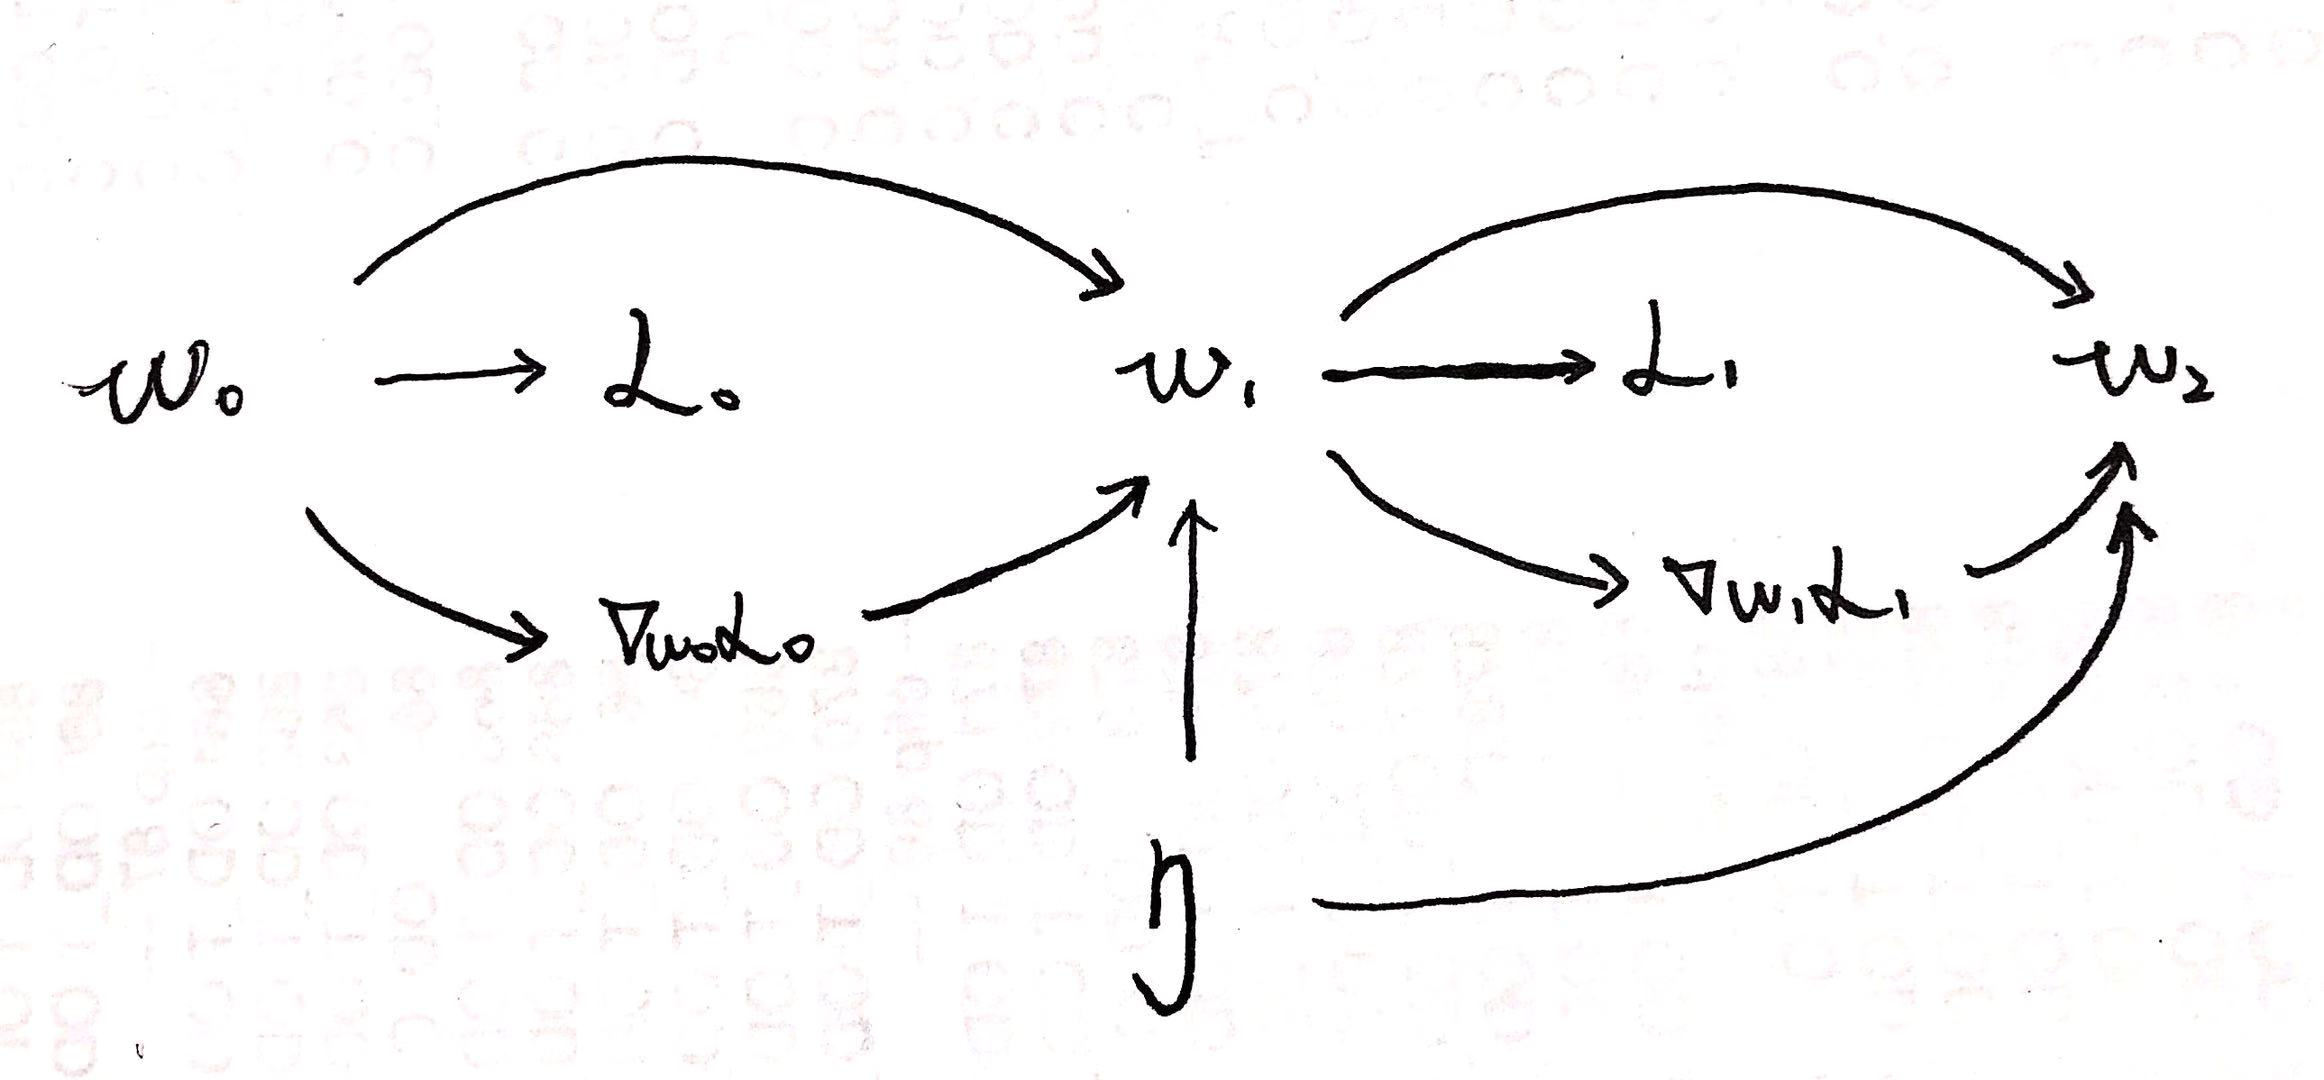
\includegraphics[width=.5\textwidth]{q2.1.1.jpeg} 
  \caption{Computation graph. }
  \label{fig:2.1.1}
\end{figure}
\\ \\
2.1.2 \emph{What is the memory complexity for the forward-propagation to compute $\mathcal{L}_t$ in terms of t? What is the memory complexity for using the standard back-propagation to compute the gradient w.r.t. the learning rate, $\nabla_{\eta} \mathcal{L}_t$ in terms of t?} \\ \\
To compute $\mathcal{L}_t$, we need to store $w_t$; 
to compute $w_t$, we need to store $w_{t-1}$ and $\nabla_{w_{t-1}} \mathcal{L}_{t-1}$. \\
The shape of $w_{t-1}$ and $\nabla_{w_{t-1}} \mathcal{L}_{t-1}$ are both $d \times 1$.\\
Thus, the memory complexity for the forward-propagation to compute $\mathcal{L}_t$ is O(d). In terms of $t$, the memory complexity for the forward-propagation is O(1). 
\begin{gather*}
\begin{aligned}
\overline{\nabla_{w_i} \mathcal{L}_i} &= - \eta \overline{w_{i+1}} \\
\overline{w_i} &= \overline{w_{i+1}} - \frac{2}{n} X^T X \overline{\nabla_{w_i} \mathcal{L}_i} 
= \overline{w_{i+1}} - \frac{2 \eta}{n} X^T X \overline{w_{i+1}} \\
\overline{\nabla_{\eta} \mathcal{L}_t} &= \sum_{i=1}^t \overline{w_i}^T \frac{\partial w_i}{\partial \eta} \\
\end{aligned}
\end{gather*}
The shape of $\overline{w_t}$ and $\overline{\nabla_{w_t} \mathcal{L}_t}$ are both $d \times 1$.\\
The memory complexity for using the standard back-propagation to compute the gradient w.r.t. $w_i$ is O(1). However, we need to store all the $\overline{w_i}$ to compute $\overline{\nabla_{\eta} \mathcal{L}_t}$.
Thus, the memory complexity for using the standard back-propagation to compute the gradient w.r.t. the learning rate is O(t). 
\\ \\
2.1.3 \emph{Explain one potential problem for applying gradient-based hyper-parameter optimization in more realistic examples where models often take many iterations to converge.} \\ 
\\
One potential problem can be that for a realistic example where models often take many iterations to converge, if the optimized learning rate $\eta_t$ becomes less with the increase of iteration $t$, the decreasing rate of $\mathcal{L}$ will also become less, which will drive the model for more iterations, i.e., take more time to converge and need more space/memory to calculate $\eta^*$. 
\end{homeworkSection}
%%% Subquestion 2
\begin{homeworkSection}
Learning Learning Rates. \\ \\
2.2.1 \emph{Write down the expression of $w_1$ in terms of $w_0$, $\eta$, $t$ and $X$. Then, using the expression to derive the loss $\mathcal{L}_1$ after single GD iteration in terms of $\eta$.} \\ \\
We have
\begin{gather*}
\begin{aligned}
\frac{\partial \mathcal{L}}{\partial w} &= \frac{2}{n} X^T(X w - t) \\
w_1 &\leftarrow w_0 - \frac{2 \eta}{n} X^T (X w_0 - t) = w_0 - \frac{2 \eta}{n} X^T a \\
\mathcal{L}_1 &= \frac{1}{n} ||X w_1 - t||_2^2 = \frac{1}{n} ||a - \frac{2 \eta}{n} X X^T a||_2^2
\end{aligned}
\end{gather*}
2.2.2 \emph{Determine if this $\mathcal{L}_1$ is convex w.r.t. the learning rate $\eta$.} 
\begin{gather*}
\begin{aligned}
\frac{\partial \mathcal{L}_1}{\partial \eta} &= \frac{4}{n^2} a^T XX^T (a-\frac{2\eta}{n}XX^Ta) \\
&= \frac{4}{n^2} a^T XX^T a - \frac{8\eta}{n^3} a^T XX^T XX^Ta\\
\frac{\partial \mathcal{L}_1^2}{\partial^2 \eta} &= \frac{8}{n^3} a^T XX^T XX^Ta = \frac{8}{n^3} ||XX^Ta||^2
\end{aligned}
\end{gather*}
As the second order derivative of $\mathcal{L}$ is positive, $\mathcal{L}_1$ is convex w.r.t. the learning rate $\eta$.
\\ \\
2.2.3 \emph{Write down the derivative of $\mathcal{L}_1$ w.r.t. $\eta$ and use it to find the optimal learning rate $\eta^*$ that minimizes the loss after one GD iteration.} 
\begin{gather*}
\begin{aligned}
\frac{\partial \mathcal{L}_1}{\partial \eta} &= 0 \\
\frac{4}{n^2} a^T XX^T a - \frac{8\eta}{n^3} a^T XX^T XX^Ta &= 0 \\
\eta^* &= \frac{n a^T XX^T a}{2 a^T XX^T XX^Ta}
\end{aligned}
\end{gather*}
\end{homeworkSection}
\end{homeworkProblem}


%% Question 3
\begin{homeworkProblem}
Convolutional Neural Networks.
%%% Subquestion 1
\begin{homeworkSection}
Convolutional Filters. \emph{Write down the values of the resulting matrix. What feature does this convolutional filter detect?} 
\begin{gather*}
\begin{aligned}
\textbf{I} * \textbf{J} = \begin{bmatrix}
-1 & 2 & 2 & -2 & 0\\
-2 & 1 & 0 & 2 & -1\\
3 & 0 & 0 & 1 & -1\\
-2 & 2 & 0 & 2 & -1\\
0 & -2 & 3 & -2 & 0
\end{bmatrix}
\end{aligned}
\end{gather*}
\end{homeworkSection}
%%% Subquestion 2
\begin{homeworkSection}
Size of ConvNets. \emph{Calculate the number of parameters for this conv net including the bias units.} \\ 
\begin{center}
\begin{tabular}[h]{ |c|c|c| } 
\hline
Layers & Output Units & Parameters \\
\hline
Image & 112*112*3 & - \\
Conv3-64 & 112*112*64 & 3*3*3*64+64=1,792 \\
MaxPool & 56*56*64 & - \\
Conv3-128 & 56*56*128 & 64*3*3*128+128=73,856 \\
MaxPool & 28*28*128 & - \\
Conv3-256 & 28*28*256 & 128*3*3*256+256=295,168 \\
Conv3-256 & 28*28*256 & 256*3*3*256+256=590,080 \\
MaxPool & 14*14*256 & - \\
FC-1024 & 1024 & 14*14*256*1024+1024=51,381,248 \\
FC-100 & 100 & 1024*100+100=102,500 \\
Soft-max & 100 & - \\
\hline
Total & - & 52,444,644 \\
\hline
\end{tabular}
\end{center}
\end{homeworkSection}
\end{homeworkProblem}

\end{document}

%\begin{gather*}
%\end{gather*}



